\documentclass[11pt,a4paper]{article}

\usepackage{graphicx}
\usepackage{fancyhdr}
\usepackage[margin=2.2cm]{geometry}
\usepackage{booktabs}
\usepackage{array}
\usepackage{colortbl}
\usepackage{multirow}
\usepackage{tikz}
\usepackage[table]{xcolor}
\usepackage{float}
\usepackage{caption}
\usepackage{enumitem}
\usepackage[most]{tcolorbox}
\usepackage[hidelinks]{hyperref}
\usepackage{xepersian}

\definecolor{ink}{RGB}{28,48,74}
\definecolor{accent}{RGB}{42,110,120}
\definecolor{okgreen}{RGB}{46,125,80}
\definecolor{failred}{RGB}{150,55,55}
\definecolor{warnamber}{RGB}{170,110,30}
\definecolor{softbg}{RGB}{246,248,250}
\definecolor{rowalt}{RGB}{242,246,248}

\hypersetup{
  colorlinks=true,
  linkcolor=accent,
  urlcolor=accent,
  citecolor=accent
}

\settextfont[Path={./font/}, Scale=1.28]{IRLotus}
\setlatintextfont[Scale=0.95]{Times New Roman}
\renewcommand{\baselinestretch}{1.4}
\setlength{\parskip}{0.45em}
\setlength{\parindent}{0pt}

\pagestyle{fancy}
\fancyhf{}
\rhead{\small\color{ink} گزارش پیشرفت \lr{MARGO}}
\lhead{\small\color{ink}\thepage}
\renewcommand{\headrulewidth}{0.8pt}
\renewcommand{\footrulewidth}{0pt}
\setlength{\headheight}{16pt}

\captionsetup{font=small, labelfont={bf,color=ink}}
\setlist[itemize]{leftmargin=1.35em, itemsep=0.3em}
\setlist[enumerate]{leftmargin=1.55em, itemsep=0.3em}
\setlist[description]{style=nextline, leftmargin=1.2em, font=\bfseries\color{ink}}

\newtcolorbox{notebox}{%
  colback=softbg, colframe=ink!75!black,
  fonttitle=\bfseries, title=نکته,
  boxrule=0.65pt, arc=1pt, left=7pt, right=7pt, top=3pt, bottom=3pt
}
\newtcolorbox{warnbox}{%
  colback=orange!5!white, colframe=warnamber,
  fonttitle=\bfseries\color{warnamber}, title=هشدار,
  boxrule=0.65pt, arc=1pt, left=7pt, right=7pt, top=3pt, bottom=3pt
}
\newtcolorbox{verdictbox}[1]{%
  colback=#1!4!white, colframe=#1!70!black,
  fonttitle=\bfseries, title=حکم,
  boxrule=0.65pt, arc=1pt, left=7pt, right=7pt, top=3pt, bottom=3pt
}

\newcommand{\T}{\lr{T}}
\newcommand{\passpill}{\textcolor{okgreen}{\textbf{قبول}}}
\newcommand{\failpill}{\textcolor{failred}{\textbf{رد}}}
\newcommand{\parkpill}{\textcolor{warnamber}{\textbf{متوقف}}}

\AtBeginDocument{
  \def\sectionautorefname{بخش}%
  \def\subsectionautorefname{زیربخش}%
  \def\figureautorefname{شکل}%
  \def\tableautorefname{جدول}%
}

\begin{document}

\begin{titlepage}
\thispagestyle{empty}
\definecolor{coverink}{RGB}{22,40,68}
\definecolor{coveraccent}{RGB}{210,180,120}
\begin{tikzpicture}[remember picture,overlay]
  \fill[coverink] (current page.south west) rectangle (current page.north east);
  \foreach \x in {-2,-1,...,16} {
    \draw[coveraccent, opacity=0.07, line width=0.4pt]
      ([xshift=\x cm]current page.south west) -- ++(0,1.25\paperheight);
  }
  \foreach \y in {-2,-1,...,22} {
    \draw[coveraccent, opacity=0.05, line width=0.35pt]
      ([yshift=\y cm]current page.south west) -- ++(1.25\paperwidth,0);
  }
  \foreach \i in {1,...,90} {
    \pgfmathsetmacro{\rx}{rnd*\paperwidth}
    \pgfmathsetmacro{\ry}{rnd*\paperheight}
    \fill[coveraccent, opacity=0.08]
      ([xshift=\rx, yshift=\ry]current page.south west) circle (0.6pt);
  }
  \fill[coveraccent, opacity=0.85]
    ([yshift=-2.1cm]current page.north west) rectangle
    ([yshift=-2.18cm]current page.north east);
  \fill[coveraccent, opacity=0.55]
    ([yshift=2.1cm]current page.south west) rectangle
    ([yshift=2.18cm]current page.south east);
\end{tikzpicture}

\vspace*{4.2cm}
\begin{center}
{\color{white}\fontsize{28}{34}\selectfont گزارش پیشرفت}\\[0.7cm]
{\color{coveraccent}\fontsize{34}{40}\selectfont\lr{MARGO}}\\[0.55cm]
{\color{white!88}\Large آزمایش‌ها، نتایج عددی و وضعیت فعلی}\\[1.1cm]
{\color{coveraccent!90}\rule{0.28\textwidth}{0.7pt}}
\end{center}

\vspace*{3.6cm}
\begin{center}
\color{white!92}\large
\begin{tabular}{rl}
تاریخ: & ۲۱ شهریور ۱۴۰۵ \\[0.25em]
نوع گزارش: & پیشرفت پژوهشی میانی \\[0.25em]
دامنهٔ ارزیابی: & مجموعهٔ اعتبارسنجی \\
\end{tabular}
\end{center}

\vfill
\vspace*{1.8cm}
\end{titlepage}
\clearpage


\tableofcontents
\clearpage
\listoffigures
\clearpage
\listoftables
\clearpage

%% ============================================================
\section{این گزارش چیست؟}
\label{sec:what}

این سند وضعیت پروژهٔ \lr{MARGO} را تا ۲۱ شهریور ۱۴۰۵ جمع می‌کند:
مسئلهٔ دقیق چیست، چه آزمایش‌هایی انجام شده، هر فاز چه گیتی داشت،
چه عددی به‌دست آمده، چه مسیرهایی رد شده‌اند، و روش پیشنهادی فعلی چیست.

\begin{warnbox}
همهٔ اعداد این گزارش روی \textbf{مجموعهٔ اعتبارسنجی} (۵ توزیع، ۵۰۰ گراف) یا
پروفایل‌های نگه‌داشته‌شده/منجمد گزارش شده‌اند.
ارزیابی نهایی روی مجموعهٔ آزمونِ کاملاً نگه‌داشته‌شده (۵ توزیع دیگر) هنوز انجام نشده است.
بنابراین این سند «پیشرفت میانی» است، نه نتیجهٔ قطعی مقاله.
\end{warnbox}

\begin{figure}[H]
\centering
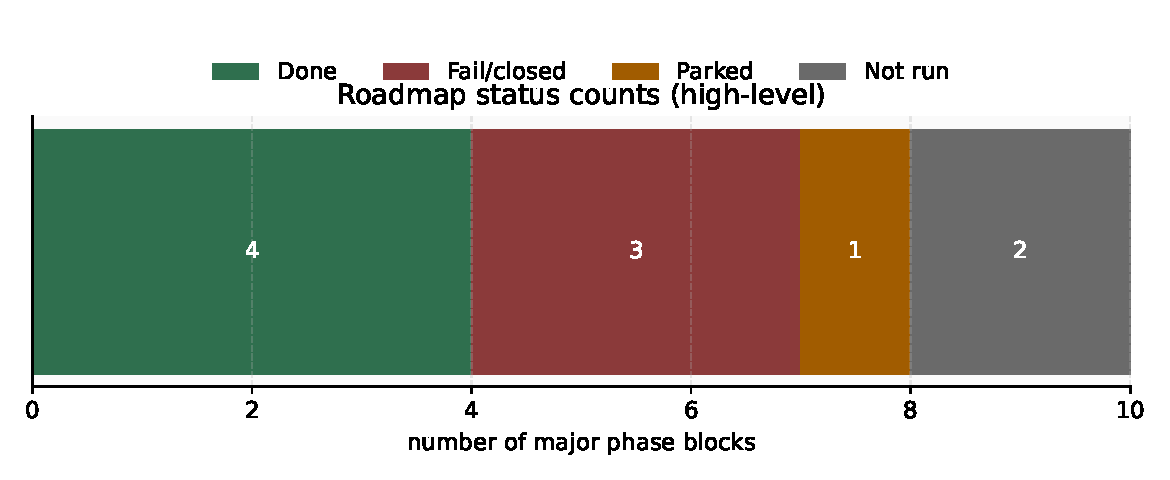
\includegraphics[width=0.92\textwidth]{img/charts/fig_roadmap.pdf}
\caption{وضعیت درشت بلوک‌های مسیر کار.}
\label{fig:roadmap}
\end{figure}

%% ============================================================
\section{مسئله و خط لوله}
\label{sec:problem}

\subsection{ورودی و خروجی}

\lr{MARGO} برای \textbf{زمان‌بندی برون‌سپاری وظایف} روی یک گراف وابستگی (\lr{DAG}) طراحی شده است.
هر نمونهٔ آزمایش یک \lr{DAG} با \textbf{۲۰ وظیفه} است؛ یال‌ها ترتیب اجرا را مشخص می‌کنند.
برای هر وظیفه باید یکی از سه اقدام انتخاب شود:

\begin{itemize}
  \item \textbf{محلی} (\lr{0}): اجرا روی گوشی (\lr{UE})
  \item \textbf{لبهٔ موبایل} (\lr{1}): ارسال به \lr{MEC}
  \item \textbf{کمک‌کنندهٔ نزدیک} (\lr{2}): ارسال از طریق \lr{V2V} به دستگاه کمکی
\end{itemize}

خروجی یک \textbf{برنامهٔ بیست‌اقدامی} است.
زمان‌بند رسمی با تقویم منابع و جدول مسیر سه‌درسه، زمان پایان کل گراف را حساب می‌کند.
این مقدار \textbf{زمان پایان} (\T، \lr{makespan}) است و بر حسب \textbf{ثانیه} گزارش می‌شود؛ کمتر بهتر است.

در مسیر تأخیر، هدف کم‌کردن \T\ است.
در مسیر انرژی (فاز ۵)، هدف ترکیب وزن‌دار زمان و انرژی موبایل با پارامتر $\lambda$ است:
\[
J_\lambda = \lambda\, T_{\mathrm{norm}} + (1-\lambda)\, E_{\mathrm{norm}}.
\]
$\lambda{=}1$ یعنی فقط زمان؛ $\lambda{=}0$ یعنی فقط انرژی موبایل (گوشی + کمک‌کننده).
انرژی محاسبهٔ سرور \lr{MEC} داخل هدف نیست.

\subsection{خط لولهٔ روش پیشنهادی}

روش فعلی در سه گام خلاصه می‌شود:

\begin{enumerate}
  \item \textbf{معلم جستجویی}: روی هر گراف، از یک برنامهٔ اولیهٔ قوی (\lr{greedy\_from\_mec})
        با جستجوی \lr{2-opt} بهترین زمان ممکن را می‌سازیم (سقف اکتشاف، نه روش نهایی).
  \item \textbf{آموزش تقلید} (\lr{BC}): شبکهٔ عصبی با رمزگذار \lr{meanagg} و خوانش \lr{mean}
        برنامهٔ معلم را روی گراف‌های آموزشی یاد می‌گیرد.
        مشاهدهٔ ورودی نسخهٔ ۲ (\lr{obs v2}) علاوه بر شکل گراف، نرخ‌های ارتباطی و پردازشی پروفایل منبع را هم می‌بیند.
  \item \textbf{استنتاج با نمونه‌گیری} (\lr{best-of-k}): در آزمون، از سیاست $k$ برنامه نمونه می‌گیریم
        (با دمای نمونه‌گیری)، برای هر نمونه یک بار زمان‌بندی رسمی (\lr{schedule()}) اجرا می‌شود،
        و کم‌زمان‌ترین برنامه نگه داشته می‌شود. $k\le 64$.
\end{enumerate}

\begin{notebox}
\textbf{حریص} (\lr{greedy}) یعنی در هر گام وظیفه، اقدام با بیشترین احتمال سیاست انتخاب می‌شود — بدون نمونه‌گیری.
\textbf{نمونه‌گیری} یعنی چند برنامهٔ متفاوت از توزیع سیاست کشیده می‌شود و بهترین زمان برداشته می‌شود.
جستجوی \lr{pair}/\lr{2-opt} در زمان آزمون جزء روش نیست؛ فقط برای ساخت معلم و سقف مرجع به‌کار رفته است.
\end{notebox}

%% ============================================================
\section{واژه‌های پرتکرار}
\label{sec:glossary}

\begin{description}
  \item[\lr{DAG}] گراف جهت‌دار بدون دور؛ ۲۰ وظیفه با یال وابستگی.
  \item[توزیع] خانوادهٔ گراف با الگوی ساختاری مشخص؛ ۲۵ توزیع در مجموعهٔ کامل.
  \item[پروفایل منبع] بردار نرخ‌های ارتباطی/پردازشی که شرایط شبکه و دستگاه را مشخص می‌کند.
  \item[\lr{obs v1}] مشاهدهٔ قدیمی: فقط ویژگی‌های گراف (بدون پروفایل منبع).
  \item[\lr{obs v2}] مشاهدهٔ جدید: ۱۵ ویژگی گره + بستهٔ ورودی ۵۴ بعدی شامل پروفایل.
  \item[\T] زمان تمام‌شدن کل گراف (ثانیه).
  \item[\lr{E}] انرژی موبایل: گوشی + کمک‌کننده (ژول).
  \item[\lr{BC}] تقلید رفتاری: شبکه برنامهٔ معلم را با زیان طبقه‌بندی یاد می‌گیرد.
  \item[\lr{best-of-k}] از سیاست $k$ برنامه نمونه‌گیری و کم‌زمان‌ترین را انتخاب.
  \item[\lr{EAS}] تطبیق تکاملی سریع روی زیرمجموعهٔ کوچک پارامترها (\lr{φ}) با چند گراف پشتیبان.
  \item[\lr{CTX}/\lr{CAVIA}] زمینهٔ فراگیر: بردار $z$ از گراف‌های پشتیبان برای شرطی‌کردن سیاست.
  \item[\lr{OOD}] خارج از توزیع آموزش (اعتبارسنجی یا پروفایل دیده‌نشده).
  \item[\lr{PPO} روی وزن سیاست] یادگیری تقویتی که وزن‌های کامل شبکه را با پاداش محیط به‌روز می‌کند.
  \item[اعتبارسنجی / آزمون نهایی] اعتبارسنجی برای تصمیم میانی؛ آزمون نهایی روی ۵ توزیع نگه‌داشته‌شده و هنوز گزارش نشده.
\end{description}

%% ============================================================
\section{تقسیم داده و مرجع‌ها}
\label{sec:contracts}

\subsection{تقسیم توزیع‌های گراف}

\begin{table}[H]
\centering
\caption{تقسیم فریز ۲۵ توزیع}
\label{tab:split}
\rowcolors{2}{white}{rowalt}
\begin{tabular}{lcp{7.5cm}}
\toprule
\rowcolor{ink!12} بخش & تعداد & شناسهٔ توزیع‌ها \\
\midrule
آموزش & ۱۵ & $\{1,3,4,5,8,9,11,13,15,18,19,21,22,24,25\}$ \\
اعتبارسنجی & ۵ & $\{2,6,10,16,17\}$ \\
آزمون نهایی & ۵ & $\{7,12,14,20,23\}$ — هنوز ارزیابی نشده \\
\bottomrule
\end{tabular}
\end{table}

هر توزیع در آموزش ۱۰۰ گراف دارد.
اعتبارسنجی ۵۰۰ گراف (۵ توزیع $\times$ ۱۰۰) است.
واحد همهٔ زمان‌ها \textbf{ثانیه} و انرژی \textbf{ژول} است.

\subsection{محور پروفایل منبع (فاز ۴)}

علاوه بر محور «شکل \lr{DAG}»، محور دوم «پروفایل منبع» اضافه شد:
گرید ۴۵ پروفایل؛ ۱۳ تای آموزش، ۲ تای نگه‌داشته‌شده (\lr{p\_5}, \lr{p\_9}),
یک پروفایل منجمد برای پیوستگی با گذشته (\lr{frozen\_7\_5\_10})،
و ۸ تای آزمون نهایی که هنوز استفاده نشده‌اند.

\subsection{کنترل مرجع \lr{A}}

کنترل \lr{A} همان \lr{BC} قدیمی روی مشاهدهٔ نسخهٔ ۱ (\lr{obs v1}) است:
حریص اعتبارسنجی \textbf{۵۷۵٫۱} ثانیه، آزمون نهایی \textbf{۵۵۷} ثانیه.
نسبت اقدام‌ها روی اعتبارسنجی حدود ۲۱٪ محلی / ۷۵٪ \lr{MEC} / ۴٪ کمک‌کننده.
روش‌های جدید معمولاً با این خط‌کش سنجیده می‌شوند.

\subsection{مرجع‌های اکتشافی}

\begin{table}[H]
\centering
\caption{مرجع‌های اکتشافی (اعتبارسنجی مگر ذکر شود)}
\label{tab:heuristics}
\rowcolors{2}{white}{rowalt}
\begin{tabular}{lcc}
\toprule
\rowcolor{ink!12} مرجع & $T$ (ثانیه) & نقش \\
\midrule
همه روی \lr{MEC} & ۶۳۴ & کف تنک‌نبودن؛ اگر سیاست تنبل شود به اینجا می‌چسبد \\
حریص انتشار از تهی & $\approx$۵۹۴ (آموزش) & مرجع ضعیف مقاله‌های قدیمی \\
حریص از مبدأ \lr{MEC} & ۴۶۴ & اکتشاف قوی بدون یادگیری \\
\lr{2-opt} از حریص \lr{MEC} & ۴۲۴ & بهترین معلم جستجویی \\
جستجوی جفت $k{=}50$ & ۴۳۸٫۹ & سقف «اکتشاف + جستجو»؛ \textbf{روش نیست} \\
\bottomrule
\end{tabular}
\end{table}

سقف فیزیکی مسئله حدود \textbf{۴۳۹} ثانیه است (\lr{h} + جستجو).
یک‌گذر \lr{LSTM} بدون جستجو روی \lr{OOD} قدیمی حدود \textbf{۵۷۵} ثانیه می‌ماند.

%% ============================================================
\section{خلاصهٔ وضعیت فازها}
\label{sec:summary}

\begin{table}[H]
\centering
\caption{فازها، گیت و نتیجه}
\label{tab:phases}
\rowcolors{2}{white}{rowalt}
\begin{tabular}{>{\raggedright\arraybackslash}p{2.8cm}c>{\raggedright\arraybackslash}p{4.2cm}>{\raggedright\arraybackslash}p{4.8cm}}
\toprule
\rowcolor{ink!12} فاز & وضعیت & گیت & نتیجهٔ عددی \\
\midrule
۰ مشخصات & \passpill & قراردادها تثبیت & مسئله، متریک، تقسیم داده فریز شد \\
۱ رمزگذار & \passpill & $\Delta T<10$ برای مدل سنگین‌تر & \lr{meanagg} بهتر از \lr{gatv2}/\lr{dagformer} \\
۲ نمونه‌گیری & \passpill & $T_{32}\le 510$ & \textbf{۵۰۹٫۱۲$\pm$۰٫۴۸} (۳ بذر) \\
۳ \lr{EAS} & \failpill & پرس‌وجو $\le 520$ & ۵۷۷٫۷$\to$۵۷۶٫۴؛ رد \\
۳ب \lr{EAS} نمونه‌ای & \failpill & $\Delta\ge 5$s vs \lr{BOK} & $-0.2$s؛ رد \\
۴ محور منبع & \passpill\ (بذر۰) & پیوستگی + نمونه‌گیری $\ge 10$s & حریص ۴۹۳٫۸؛ $T_{32}$ ۴۴۷٫۷ \\
۵ انرژی & \parkpill & فیزیک + دود & فیزیک قبول؛ معلم کامل ۱/۶۵ \\
کنترل \lr{PPO} ۵۰۰ & اجرا نشده & بستن فرضیهٔ بودجه & — \\
ارزیابی نهایی & باقی‌مانده & ۵ بذر + آزمون نهایی & — \\
\bottomrule
\end{tabular}
\end{table}

%% ============================================================
\section{چرا \lr{PPO} روی وزن سیاست کنار رفت؟}
\label{sec:c2}

فرضیهٔ اولیه: با یادگیری تقویتی (\lr{PPO}) روی وزن‌های کامل شبکه،
سیاست بهتر از معلم اکتشافی شود.
هفت پیکربندی مختلف آزمایش شد.
الگوی تکراری: سیاست کم‌کم تقریباً همه‌چیز را به \lr{MEC} می‌فرستد (\textbf{فروپاشی اشغال})
و زمان بد می‌ماند.

\begin{table}[H]
\centering
\caption{نمونه‌های نتیجهٔ منفی \lr{PPO}}
\label{tab:c2}
\rowcolors{2}{white}{rowalt}
\begin{tabular}{>{\raggedright\arraybackslash}p{3.5cm}>{\raggedright\arraybackslash}p{9.8cm}}
\toprule
\rowcolor{ink!12} اجرا & چه دیده شد \\
\midrule
۵۰۰ تکرار موازی & از تکرار ۲۱ سهم \lr{MEC} بالای ۹۵٪؛ تا تکرار ۱۸۰ نزدیک ۱۰۰٪ \\
فقط‌تأخیر ۵۰ تکرار & زمان ۹۵۸$\to$۷۹۶؛ هیچ برنامهٔ غیر-\lr{MEC} ساخته نشد \\
\lr{BC} بعد \lr{PPO} & اول نزدیک معلم؛ تا تکرار ۹ سهم محلی ۵۵٪ و خراب \\
\lr{KL} به سیاست \lr{BC} & لنگر کافی نبود؛ \lr{KL} ۱٫۱۸$\to$۱۶؛ محلی ۲۱٪$\to$۷۴٪ \\
چندنمونه‌ای با \lr{PPO} & اعتبارسنجی ۵۸۰$\to$۶۵۷ (بدتر) \\
\lr{BC} فقط ارزیابی & بازنمایی خراب نیست؛ آموزش ۵۳۳ vs معلم ۴۴۸ — مشکل انتقال \lr{OOD} است \\
\bottomrule
\end{tabular}
\end{table}

در مقابل، \textbf{تقلید در‌توزیع کار می‌کند}:
\lr{bc\_continue} روی آموزش حریص \textbf{۴۶۴} ثانیه و دقت نشانهٔ \textbf{۰٫۹۶۸} گرفت.
یعنی شبکه می‌تواند معلم را در توزیع آموزش یاد بگیرد؛
اما بهبود با پاداش روی وزن کامل در این کدپایه خراب می‌کند.

\begin{verdictbox}{failred}
\lr{PPO} روی وزن سیاست از روش حذف شد.
گیت باقی: کنترل ۵۰۰ تکرار از صفر (بدون انرژی) برای بستن فرضیهٔ «بودجهٔ کوتاه کافی نبود».
\end{verdictbox}

%% ============================================================
\section{مسیرهای رد‌شدهٔ دیگر}
\label{sec:closed}

قبل از رسیدن به روش فعلی، چند مسیر دیگر هم آزمایش و رد شد:

\begin{table}[H]
\centering
\caption{خلاصهٔ مسیرهای بسته‌شده}
\label{tab:closed}
\rowcolors{2}{white}{rowalt}
\begin{tabular}{>{\raggedright\arraybackslash}p{3.2cm}c>{\raggedright\arraybackslash}p{7.8cm}}
\toprule
\rowcolor{ink!12} مسیر & حکم & توضیح \\
\midrule
\lr{CAVIA} روی $z$ & رد & سه اجرا: پرس‌ژو ۵۸۴٫۵$\to$۵۸۵٫۱؛ ۵۸۴٫۵$\to$۵۸۴٫۲؛ ۵۷۲٫۷$\to$۵۷۲٫۷ \\
بازنویسی از \lr{all-MEC} & رد & اعتبارسنجی ۶۱۰٫۶ vs کنترل ۵۷۵؛ تقریباً هیچ جفت جایگزینی اعمال نشد \\
شناسهٔ توزیع (\lr{oracle}) & رد & هویت ۵۷۵٫۱؛ آموزش ۴۵۳٫۷ vs ۴۶۴؛ اعتبارسنجی ۵۸۴٫۲ vs ۵۷۵ \\
جفت‌آموزی (\lr{pairsup}) & رد & فقط ۷٪ جفت مثبت؛ بدون بهبود \lr{OOD} \\
\bottomrule
\end{tabular}
\end{table}

\begin{notebox}
شکاف اصلی \lr{OOD} (حدود ۵۷۵$\to$۴۳۹) از «شناسایی توزیع» یا «بازنویسی عصبی از \lr{all-MEC}» نیست،
بلکه از \textbf{وابستگی‌های مشترک داخل یک گراف} است که یک‌گذر \lr{LSTM} استخراج نمی‌کند.
جستجوی \lr{2-opt} این وابستگی‌ها را می‌بندد؛ نمونه‌گیری بخشی از آن را ارزان می‌گیرد.
\end{notebox}

%% ============================================================
\section{فاز ۱ — آیا رمزگذار ضعیف بود؟}
\label{sec:encoder}

\textbf{سؤال}: اگر شکاف \lr{OOD} از ضعف نمایش گراف باشد، رمزگذار قوی‌تر (\lr{gatv2}, \lr{dagformer})
باید زمان اعتبارسنجی را بهتر کند.

\textbf{طراحی}: سه رمزگذار، سه بذر، خوانش \lr{triple} (پیش‌فرض).
ارزیابی روی ۵۰۰ گراف اعتبارسنجی.

\begin{table}[H]
\centering
\caption{مقایسهٔ رمزگذارها (خوانش \lr{triple}، ۳ بذر)}
\label{tab:encoder}
\rowcolors{2}{white}{rowalt}
\begin{tabular}{lrrrr}
\toprule
\rowcolor{ink!12} رمزگذار & پارامتر & میانگین $T$ & انحراف & $\Delta T$ \\
\midrule
\lr{meanagg} & ۴۲۹۱۸۵ & $\mathbf{588.78}$ & $\pm 11.83$ & — \\
\lr{gatv2} & ۶۲۶۸۱۷ & ۶۰۰.۵۴ & $\pm 4.29$ & $-11.8$ (بدتر) \\
\lr{dagformer} & ۵۳۱۰۷۳ & ۵۹۷.۳۳ & $\pm 2.84$ & $-8.6$ (بدتر) \\
\bottomrule
\end{tabular}
\end{table}

هر دو رقیب سنگین‌تر \textbf{بدتر} شدند؛ گیت $\Delta T < 10$ برای هر دو (هر دو منفی) →
شکاف \lr{OOD} نمایشی نیست.

\subsection{آزمایش نوع خوانش}

روی \lr{meanagg} بذر صفر، خوانش \lr{mean} از \lr{triple} حدود ۱۱ ثانیه بهتر بود:

\begin{table}[H]
\centering
\caption{نوع خوانش روی \lr{meanagg} بذر ۰}
\label{tab:readout}
\rowcolors{2}{white}{rowalt}
\begin{tabular}{lcc}
\toprule
\rowcolor{ink!12} خوانش & $T$ اعتبارسنجی & اختلاف با \lr{triple} \\
\midrule
\lr{triple} & ۵۸۸٫۱۴ & — \\
\lr{mean} & $\mathbf{577.02}$ & $-11.1$ \\
\lr{attn} & ۵۸۳٫۰۸ & $-5.1$ \\
\lr{max} & ۵۹۳٫۹۴ & $+5.8$ \\
\lr{zero} & ۵۹۵٫۰۰ & $+6.9$ \\
\bottomrule
\end{tabular}
\end{table}

\begin{figure}[H]
\centering
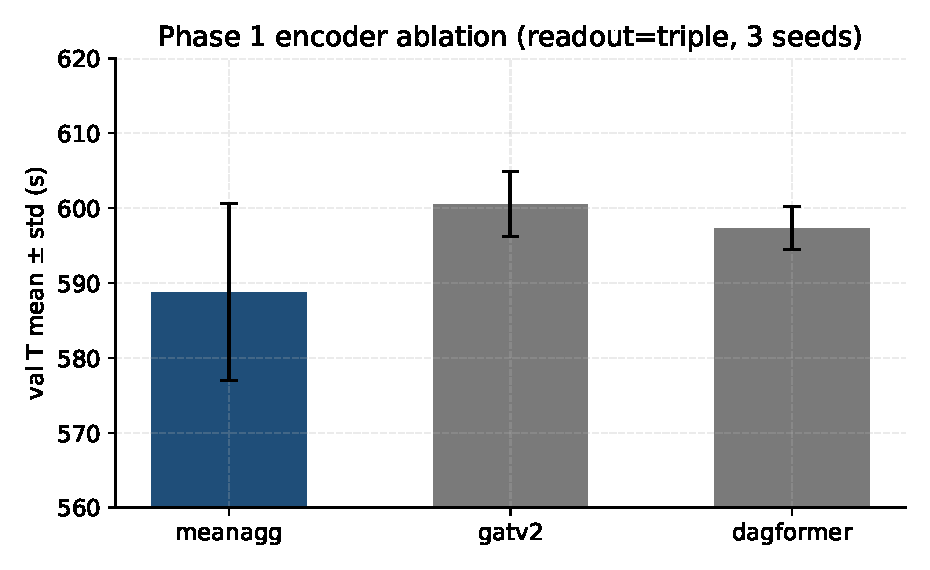
\includegraphics[width=0.78\textwidth]{img/charts/fig_encoder.pdf}
\caption{مقایسهٔ رمزگذارها.}
\label{fig:encoder}
\end{figure}

\begin{verdictbox}{okgreen}
رمزگذار نهایی: \lr{meanagg} + خوانش \lr{mean}.
شکاف \lr{OOD} از «نمایش گراف» نیست.
\end{verdictbox}

%% ============================================================
\section{فاز ۲ — نمونه‌گیری چندبرنامه}
\label{sec:bok2}

\textbf{سؤال}: بدون آموزش تازه، آیا نمونه‌گیری از سیاست \lr{BC} زمان \lr{OOD} را پایین می‌آورد؟

\textbf{طراحی}: وزنهٔ \lr{meanagg\_triple} بذر ۰ (بدون آموزش مجدد).
روی ۵۰۰ گراف اعتبارسنجی، $k$ برنامه نمونه و بهترین \T\ گزارش می‌شود.
سه بذر برای میانگین و انحراف.

\begin{table}[H]
\centering
\caption{\lr{best-of-k} روی اعتبارسنجی}
\label{tab:bok2}
\rowcolors{2}{white}{rowalt}
\begin{tabular}{cccccc}
\toprule
\rowcolor{ink!12} $k$ & ارزیابی/گراف & بذر ۰ & بذر ۱ & بذر ۲ & میانگین$\pm$انحراف \\
\midrule
۱ & ۱ & ۵۸۸٫۱۴ & ۵۸۸٫۱۴ & ۵۸۸٫۱۴ & ۵۸۸٫۱۴$\pm$۰ \\
۸ & ۸ & ۵۳۳٫۰۱ & ۵۳۲٫۵۰ & ۵۳۱٫۱۶ & ۵۳۲٫۲۳$\pm$۰٫۹۶ \\
۳۲ & ۳۲ & ۵۰۸٫۹۳ & ۵۰۹٫۶۷ & ۵۰۸٫۷۶ & $\mathbf{509.12\pm0.48}$ \\
۶۴ & ۶۴ & ۵۰۱٫۶۹ & ۵۰۱٫۸۰ & ۵۰۱٫۱۲ & ۵۰۱٫۵۴$\pm$۰٫۳۷ \\
\bottomrule
\end{tabular}
\end{table}

گیت $T_{32} \le 510$: \passpill\ در هر سه بذر.
بهبود نسبت به حریص: حدود \textbf{۸۶٫۶} ثانیه ($k{=}64$).
روی آموزش $T_{64}$ حدود \textbf{۴۱۵٫۴} (معلم \lr{2-opt} آموزش ۴۱۴٫۱).

\textbf{اما} به سقف معلم \lr{2-opt} (۴۲۴) نمی‌رسد.
اوراکل درون نمونه‌ها: با $k{=}64$ تقریباً \textbf{۰٫۰۲۲} ثانیه بهتر از \lr{2-opt} — یعنی نمونه‌ها تقریباً هرگز معلم را نمی‌زنند.

\textbf{دمای نمونه‌گیری} ($k{=}32$): دمای ۰٫۷ → ۵۱۹٫۹ (بدتر)؛ ۱٫۰ → ۵۰۹٫۱؛ ۱٫۳ → ۵۰۲٫۳ (بهتر ولی تکراری زیاد).

\begin{figure}[H]
\centering
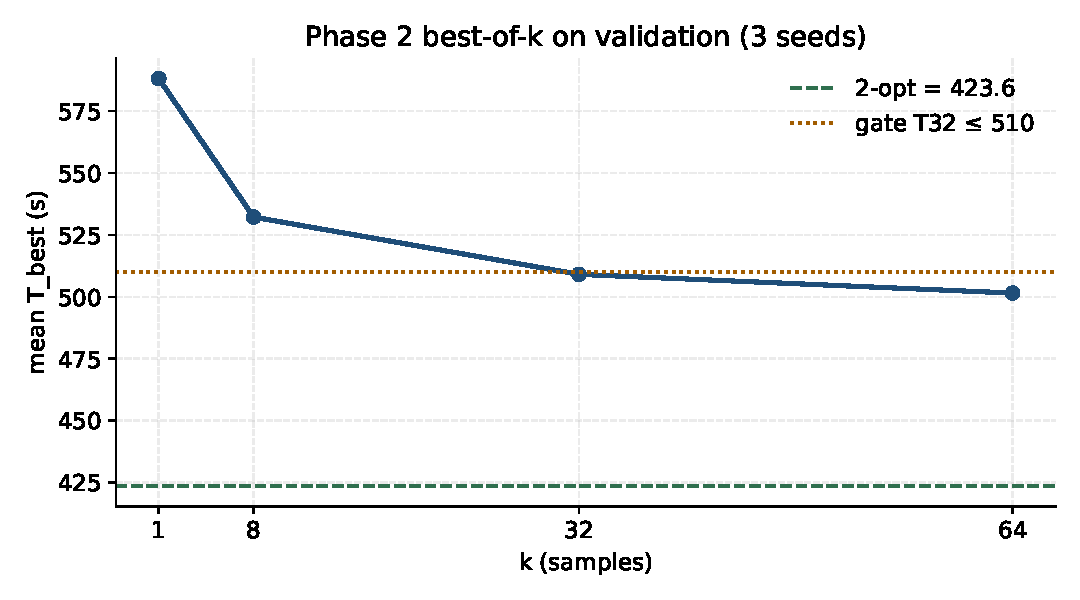
\includegraphics[width=0.82\textwidth]{img/charts/fig_bok_phase2.pdf}
\caption{اثر $k$ در فاز ۲؛ خط سبز سقف معلم.}
\label{fig:bok2}
\end{figure}

%% ============================================================
\section{فاز ۳ — تطبیق سریع (\lr{EAS})}
\label{sec:adapt}

\textbf{سؤال}: آیا با ۲۰ گراف پشتیبان از یک توزیع،
تطبیق تکاملی روی ۳۸۴ پارامتر آخر (\lr{φ}) پرس‌وجو را بهتر می‌کند؟

\textbf{پیکربندی اصلی} (\lr{lastlayer} + \lr{pg\_il}، بذر ۰):
\begin{itemize}
  \item پرس‌ژوی حریص: ۵۷۷٫۷$\to$۵۷۶٫۴ ثانیه (۲ توزیع بدتر، ۳ بهتر)
  \item بهترین ابلاسیون (\lr{pg}): ۵۷۱٫۲ ثانیه — هنوز گیت $\le 520$ \failpill
  \item پشتیبان: بهترین زمان از ۵۵۹ به ۴۶۳ رسید (جستجو روی پشتیبان کار می‌کند)
\end{itemize}

\textbf{مسیر نمونه‌ای} (بودجهٔ برابر $B{=}32$، ۵۰۰ گراف):
\lr{best-of-k} \textbf{۴۹۸٫۸} vs \lr{EAS} \textbf{۴۹۸٫۶} (اختلاف $-0.2$ ثانیه) — گیت $\ge 5$s \failpill.

\textbf{\lr{CAVIA}} (سه اجرای قبلی): پرس‌ژو تقریباً تخت؛ $z$ استفاده نمی‌شود.

\begin{figure}[H]
\centering
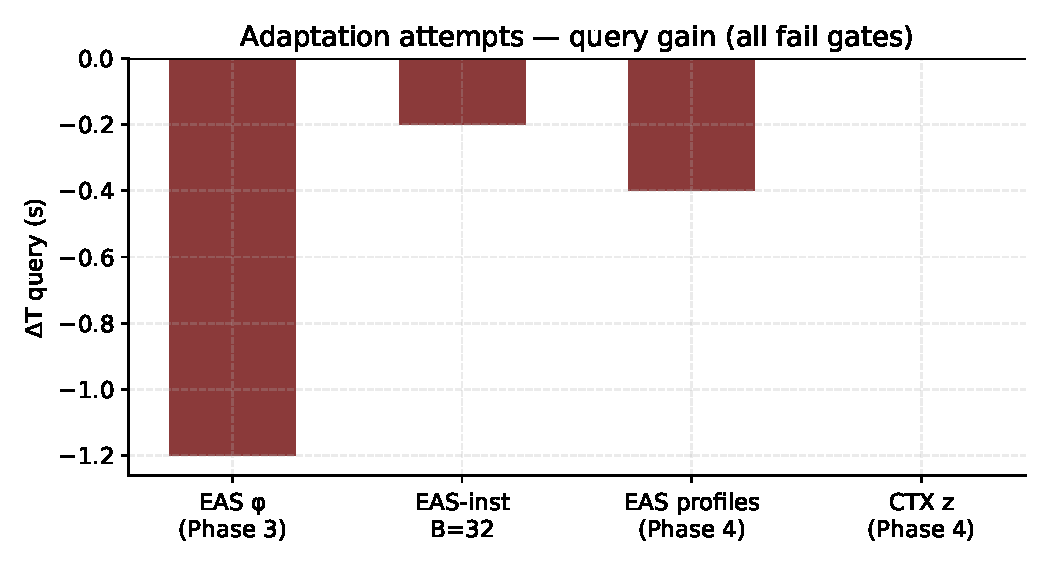
\includegraphics[width=0.82\textwidth]{img/charts/fig_adapt_fail.pdf}
\caption{سود پرس‌ژو در تلاش‌های تطبیق؛ همه نزدیک صفر.}
\label{fig:adapt}
\end{figure}

\begin{verdictbox}{failred}
تطبیق سطح‌توزیع (\lr{EAS}) و زمینهٔ فراگیر (\lr{CAVIA}) از روش حذف شدند.
روش = تقلید + نمونه‌گیری.
\end{verdictbox}

%% ============================================================
\section{فاز ۴ — محور پروفایل منبع}
\label{sec:phase4}

\textbf{سؤال}: اگر شبکه نرخ‌های ارتباطی/پردازشی پروفایل را هم ببیند (\lr{obs v2})،
آیا \lr{OOD} بهتر می‌شود؟

\subsection{آماده‌سازی}

\begin{itemize}
  \item مشاهدهٔ نسخهٔ ۲: \textbf{۱۵} ویژگی گره، بستهٔ \textbf{۵۴} بعدی
  \item آمار نرمال‌سازی از \textbf{۱۹۵۰۰} گراف آموزشی
  \item معلم \lr{2-opt} برای ۱۳ پروفایل آموزشی: حدود ۲۲ دقیقه
  \item پروفایل منجمد: \lr{2-opt} آموزش \textbf{۴۱۴٫۱} / اعتبارسنجی \textbf{۴۲۳٫۶}
\end{itemize}

\subsection{آموزش \lr{BC} با پروفایل (بذر ۰)}

۱۲۰ دوره، ۱۹۵۰۰ گراف، حدود ۱۵۲ دقیقه.
روی پروفایل منجمد:
\begin{itemize}
  \item حریص: \textbf{۴۹۳٫۸} ثانیه (قبلاً فاز ۱ بدون پروفایل: \textbf{۵۷۷٫۰}؛ بهبود \textbf{۸۳٫۲} ثانیه)
  \item نسبت اقدام‌ها با معلم هم‌خوان
  \item گیت پیوستگی یک‌طرفه (بدتر نشدن): \passpill
\end{itemize}

\subsection{نمونه‌گیری روی پروفایل منجمد}

\begin{table}[H]
\centering
\caption{\lr{best-of-k} فاز ۴ — پروفایل منجمد، ۵۰۰ گراف}
\label{tab:bok4}
\rowcolors{2}{white}{rowalt}
\begin{tabular}{cccc}
\toprule
\rowcolor{ink!12} $k$ & $T_{\mathrm{best}}$ & نسبت به حریص & فاصله تا \lr{2-opt} \\
\midrule
۱ & ۴۹۳٫۸۲ & ۰ & $+70.2$ \\
۸ & ۴۵۹٫۳۹ & $-34.4$ & $+35.8$ \\
۳۲ & $\mathbf{447.67}$ & $-46.2$ & $+24.0$ \\
۶۴ & $\mathbf{444.48}$ & $-49.3$ & $+20.9$ \\
\bottomrule
\end{tabular}
\end{table}

نسبت اقدام حریص منجمد: محلی \textbf{۲۲٫۶٪} / \lr{MEC} \textbf{۷۰٫۳٪} / کمک‌کننده \textbf{۷٫۲٪}.

\subsection{پروفایل‌های نگه‌داشته‌شده}

\begin{table}[H]
\centering
\caption{پروفایل‌های دیده‌نشده در آموزش}
\label{tab:heldout}
\rowcolors{2}{white}{rowalt}
\begin{tabular}{lcccc}
\toprule
\rowcolor{ink!12} پروفایل & حریص & $T_{64}$ & معلم \lr{2-opt} & دقت نشانه \\
\midrule
\lr{p\_5} & ۶۲۱٫۸ & ۵۴۶٫۹ & ۵۱۶٫۹ & ۰٫۶۷۰ \\
\lr{p\_9} & ۴۱۸٫۴ & ۳۷۷٫۹ & ۳۶۳٫۶ & ۰٫۷۳۷ \\
\lr{frozen} & ۴۹۳٫۸ & ۴۴۴٫۵ & ۴۲۳٫۶ & — \\
\bottomrule
\end{tabular}
\end{table}

\textbf{\lr{EAS} روی پروفایل} (بذر ۰): $T_0$ ۵۲۱٫۱$\to T^*$ ۵۲۱٫۵ ($\Delta -0.4$s) — \failpill.

\textbf{\lr{CTX} روی پروفایل} (بذر ۰): $T_0$ ۵۲۸٫۲$= T_{\mathrm{ctx}}$ ۵۲۸٫۲ ($\Delta$ ۰) — \failpill.

\begin{figure}[H]
\centering
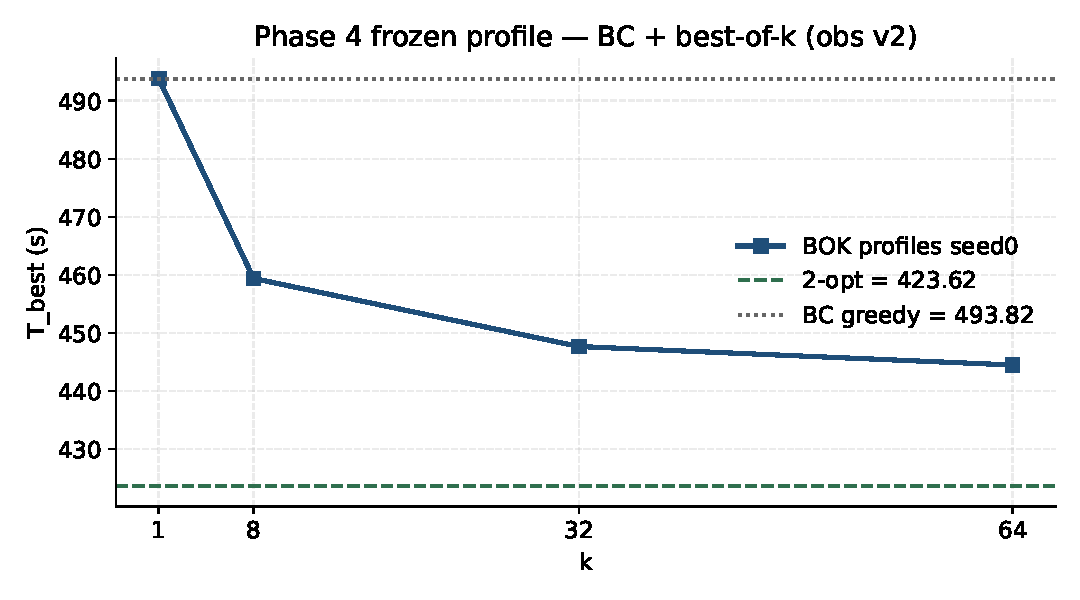
\includegraphics[width=0.82\textwidth]{img/charts/fig_bok_phase4.pdf}
\caption{نمونه‌گیری فاز ۴.}
\label{fig:bok4}
\end{figure}

\begin{figure}[H]
\centering
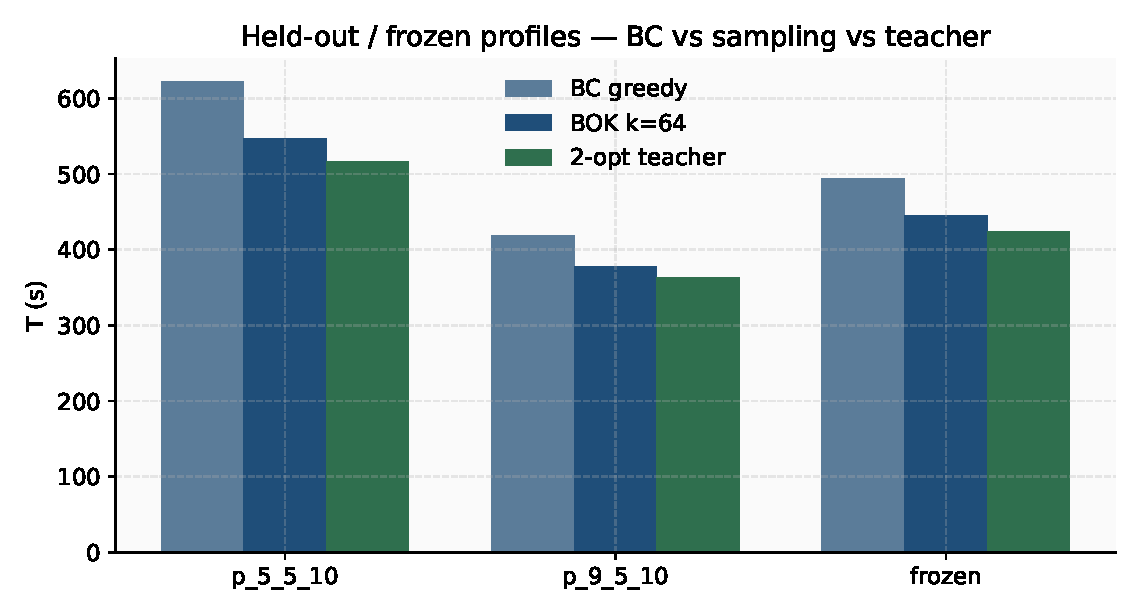
\includegraphics[width=0.86\textwidth]{img/charts/fig_heldout.pdf}
\caption{پروفایل‌های نگه‌داشته‌شده و منجمد.}
\label{fig:heldout}
\end{figure}

\begin{warnbox}
محور منبع فعلاً فقط \textbf{بذر صفر} کامل است.
بذرهای ۱ و ۲ برای \lr{BC} و نمونه‌گیری هنوز اجرا نشده‌اند؛
میانگین و انحراف چندبذری این محور گزارش نشده است.
\end{warnbox}

%% ============================================================
\section{نردبان زمان}
\label{sec:ladder}

شکل و جدول زیر همهٔ روش‌ها را در یک قاب می‌نشانند (اعتبارسنجی، ثانیه؛ کمتر بهتر):

\begin{figure}[H]
\centering
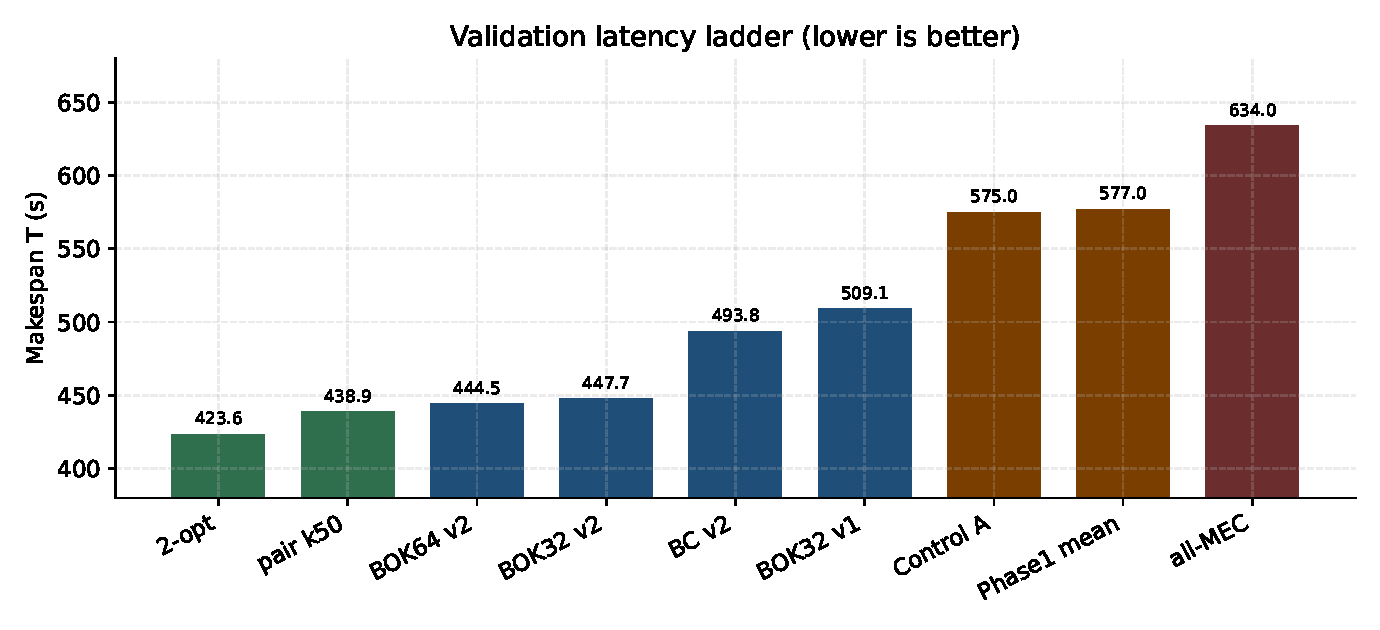
\includegraphics[width=0.95\textwidth]{img/charts/fig_t_ladder.pdf}
\caption{نردبان زمان.}
\label{fig:ladder}
\end{figure}

\begin{table}[H]
\centering
\caption{نردبان عددی}
\label{tab:ladder}
\rowcolors{2}{white}{rowalt}
\begin{tabular}{lc}
\toprule
\rowcolor{ink!12} روش / مرجع & $T$ (ثانیه) \\
\midrule
معلم \lr{2-opt} & ۴۲۳٫۶ \\
جستجوی جفت $k{=}50$ & ۴۳۸٫۹ \\
نمونه‌گیری $k{=}64$ فاز ۴ (بذر ۰) & ۴۴۴٫۵ \\
نمونه‌گیری $k{=}32$ فاز ۴ (بذر ۰) & ۴۴۷٫۷ \\
\lr{BC} حریص فاز ۴ (بذر ۰) & ۴۹۳٫۸ \\
نمونه‌گیری $k{=}32$ فاز ۲ (۳ بذر) & ۵۰۹٫۱ \\
کنترل \lr{A} (\lr{obs v1}) & ۵۷۵ \\
فاز ۱ حریص (\lr{obs v1}) & ۵۷۷ \\
همه روی \lr{MEC} & ۶۳۴ \\
\bottomrule
\end{tabular}
\end{table}

\textbf{برداشت}: مشاهدهٔ پروفایل منبع حریص را از ۵۷۷ به ۴۹۴ می‌آورد ($-83$s).
نمونه‌گیری $k{=}32$ را به ۴۴۸ می‌رساند ($-46$s دیگر).
هنوز ۲۴ ثانیه تا معلم \lr{2-opt} فاصله است.

%% ============================================================
\section{فاز ۵ — انرژی}
\label{sec:energy}

\textbf{هدف}: ساختن جبههٔ زمان–انرژی با $\lambda \in \{1, 0.75, 0.5, 0.25, 0\}$.

\textbf{آزمون‌های فیزیک} (محلی): قبول —
\lr{2-opt} با $J_{\lambda=1}$ همان \T\ \lr{2-opt} است؛
انرژی کمک‌کننده روی \lr{V2V}؛
$\lambda$ پایین $\to$ همه \lr{MEC} (چون انرژی \lr{MEC} در هدف نیست).

\textbf{دود دستی} روی ۸ گراف پروفایل منجمد:

\begin{table}[H]
\centering
\caption{دود دستی انرژی}
\label{tab:energy-smoke}
\rowcolors{2}{white}{rowalt}
\begin{tabular}{cccc}
\toprule
\rowcolor{ink!12} $\lambda$ & $T$ & $E$ (ژول) & سهم \lr{MEC} \\
\midrule
۱٫۰۰ & ۳۳۳ & ۳۱۴ & ۰٫۷۷۵ \\
۰٫۷۵ & ۳۴۱ & ۲۴۵ & ۰٫۸۳۱ \\
۰٫۵۰ & ۴۳۰ & ۷۴ & ۰٫۹۶۹ \\
۰٫۲۵ / ۰٫۰۰ & ۴۶۸ & ۳۹ & ۱٫۰۰۰ \\
\bottomrule
\end{tabular}
\end{table}

روند: با کم‌شدن $\lambda$، زمان بالا و انرژی موبایل پایین می‌آید.
در $\lambda{=}1$ اقدام‌ها با معلم تأخیر فاز ۴ یکی بود.

\textbf{تولید کامل معلم انرژی}: ۱ از ۶۵ ترکیب (پروفایل $\times$ $\lambda$) انجام شد؛ وسط کار متوقف شد.

\begin{figure}[H]
\centering
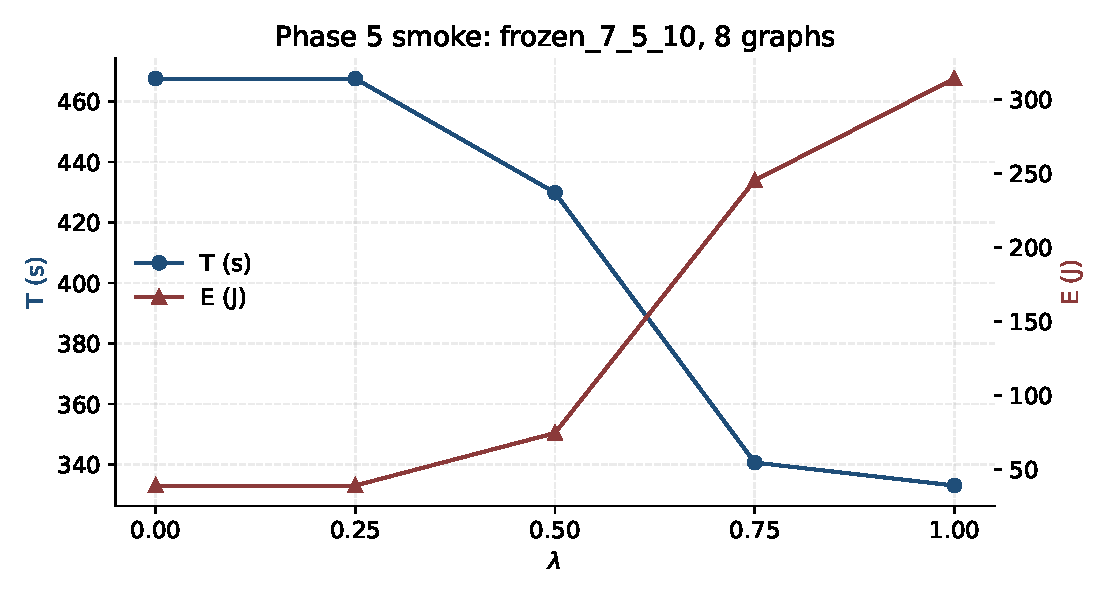
\includegraphics[width=0.82\textwidth]{img/charts/fig_energy_smoke.pdf}
\caption{دود دستی فاز ۵.}
\label{fig:energy}
\end{figure}

\begin{warnbox}
فاز ۵ \textbf{متوقف} است.
جبههٔ پارتو و آموزش سیاست شرطی‌شده روی انرژی هنوز وجود ندارد.
تا تکمیل، فقط مسیر تأخیر قابل گزارش است.
\end{warnbox}

%% ============================================================
\section{روش پیشنهادی فعلی}
\label{sec:method}

\begin{notebox}
\textbf{روش \lr{MARGO} نسخهٔ ۰٫۳} (تأخیر):
\begin{enumerate}
  \item رمزگذار \lr{meanagg} + خوانش \lr{mean}
  \item مشاهدهٔ \lr{obs v2} (گراف + پروفایل منبع)
  \item آموزش \lr{BC} از معلم \lr{2-opt}
  \item استنتاج \lr{best-of-k} با $k \le 64$ و یک \lr{schedule()} per نمونه
\end{enumerate}
بدون: \lr{PPO}، \lr{EAS}، \lr{CAVIA}، جستجوی \lr{pair}/\lr{2-opt} در آزمون.
\end{notebox}

\textbf{بهترین عدد فعلی} (اعتبارسنجی، پروفایل منجمد، بذر ۰):
$T_{64} = \mathbf{444.5}$ ثانیه (فاصله تا \lr{2-opt}: $+20.9$s).

%% ============================================================
\section{محدودیت‌های ادعا}
\label{sec:nonclaims}

با شواهد موجود، موارد زیر را \textbf{نباید} به‌عنوان نتیجهٔ نهایی مطرح کرد:
\begin{itemize}
  \item برتری قطعی نسبت به \lr{MRLCO} یا \lr{DAMRL} (پروتکل متفاوت است)
  \item نوآوری رمزگذار گرافی به‌عنوان سهم اصلی (رمزگذار ساده کافی بود)
  \item \lr{PPO}، \lr{EAS}، \lr{CAVIA} یا فراگیر‌سازی سریع به‌عنوان روش
  \item درصد بهبود نسبت به حریص انتشار ضعیف مقالات قدیمی
  \item جبههٔ پارتو انرژی آموخته‌شده
  \item هر عدد روی مجموعهٔ آزمون نهایی (هنوز ارزیابی نشده)
  \item میانگین چندبذری محور منبع (فقط بذر ۰ کامل است)
\end{itemize}

%% ============================================================
\section{گام‌های بعدی}
\label{sec:next}

\begin{enumerate}
  \item \textbf{کنترل \lr{PPO} ۵۰۰ تکرار}: از صفر، بدون انرژی — بستن فرضیهٔ کمبود بودجه
  \item \textbf{بذرهای ۱ و ۲ محور منبع}: میانگین و انحراف برای \lr{BC} و نمونه‌گیری
  \item \textbf{تکمیل معلم انرژی} (در صورت نیاز مقاله): ۶۴ ترکیب باقی‌مانده
  \item \textbf{ارزیابی نهایی}: ۵ بذر + مجموعهٔ آزمون نگه‌داشته‌شده
\end{enumerate}

\end{document}
